\documentclass[a4paper,twocolumn]{jsarticle}
\usepackage{fancyhdr}
\usepackage[top=20truemm,bottom=20truemm,left=25truemm,right=25truemm]{geometry}
\usepackage[dvipdfmx]{graphicx}
\usepackage{float}
\pagestyle{fancy}

\begin{document}
\rhead{\parbox{15zw}{区分:情報科学区分\\氏名:丹羽 英人\\現在の専門;身体運動制御学\\希望研究室:ロボティクス 研究室\\}}
    \ \\
    \ \\
    \section{課題1これまでの修学内容}
    私は大阪大学基礎工学部システム科学科機械科学コースに所属してます。弊学におきまして、材料力学・機械力学・熱力学・流体力学といった四力を中心とした機械の性質に関して学習を行いました。また、その中のロボット工学といった授業ではマニピュレータの動作理論や特異点などのロボット制御に関する理論的学習を行いました。

    また、課外活動として大阪大学公認ロボット製作団体Robohanに所属し、回路班として基板の設計・製作、C/C++を用いたベースプログラムの開発を行いました。 NHK学生ロボコン2018にはピットクルーとして参加し、全国大会出場も果たしました。また、会計やサーバ管理者として会の運営や後輩育成に力を入れました。

    さらに、大阪大学にて行われている自主研究奨励事業において、「自走式ロボットによる環境マッピングと自己位置推定」、「適応フィルタを用いた多輪システム制御器とリアルタイム軌道追従」と題し2年間かけ自律型ロボットのマッピング、自己位置推定や軌道追従に関しての研究を行いました。

    現在、私は身体運動制御学グループ西川研究室に所属してます。その中で平井先生のグループに所属し下肢の運動解析を行ってます。その中で行っている研究は2種類あり、筋シナジー情報を用いた空気圧人工筋2足ロボットの制御と機能的電気刺激(FES)を用いた下肢の身体制御です。

    まず、空気圧人工筋を用いた2足ロボットに関して、弊研究室では従来2機の2足ロボットが存在しました。1機目の2足ロボットは自転車のペダリング動作を行うロボットです。ロボット自身、無限回転を行える自転車上に固定されており腸骨より下部のみ可動となってます。本ロボットは人間のペダリング動作の解析を目的としたロボットであるため制御情報は人間より得ています。健常者と脚に障がいを負った障がい者の方の筋シナジー情報を解析することにより、各筋対における筋拮抗比・筋拮抗和の導出を行います。その導出結果よりロボットの動作情報を算出しロボットでその再現を行い健常者と障がい者の行動解析の手段として用いました。\\
    \ \\
    \\

    \begin{figure}[H]
        \centering
        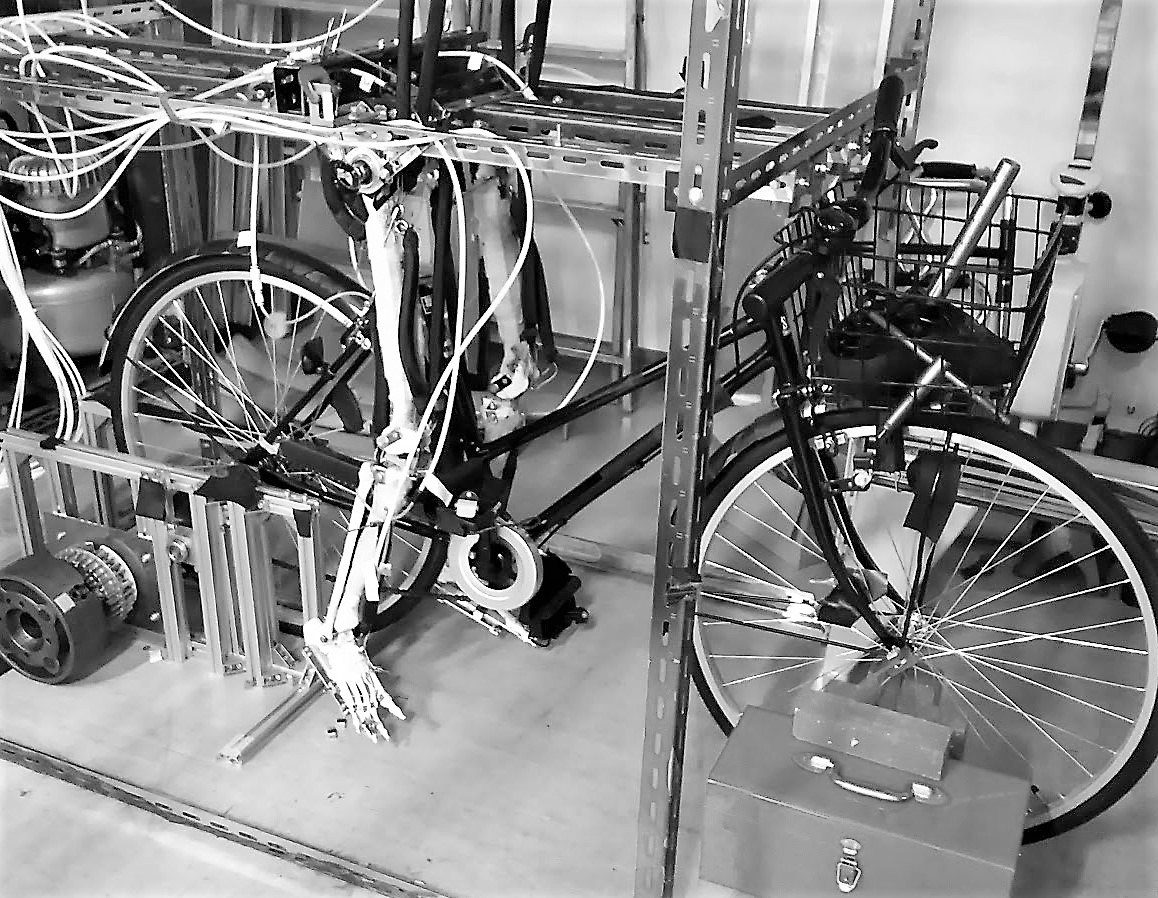
\includegraphics[width=7.5cm]{1st.jpg}
        \caption{1機目2足歩行ロボット}
    \end{figure}
    
    2機目2足ロボットは以前のロボットとは異なり人間の歩容解析を目的としたロボットです。股の部分を体重免荷装置にて支えることによってバランスの保持を行ってます。体重免荷装置の下にある、トレッドミルによって歩容環境の再現を行いました。先述の条件下において先行研究例と同様に健常者と障がい者の歩容の比較を行い障がい者における歩容変化の解析を行いました。

    \begin{figure}[H]
        \centering
        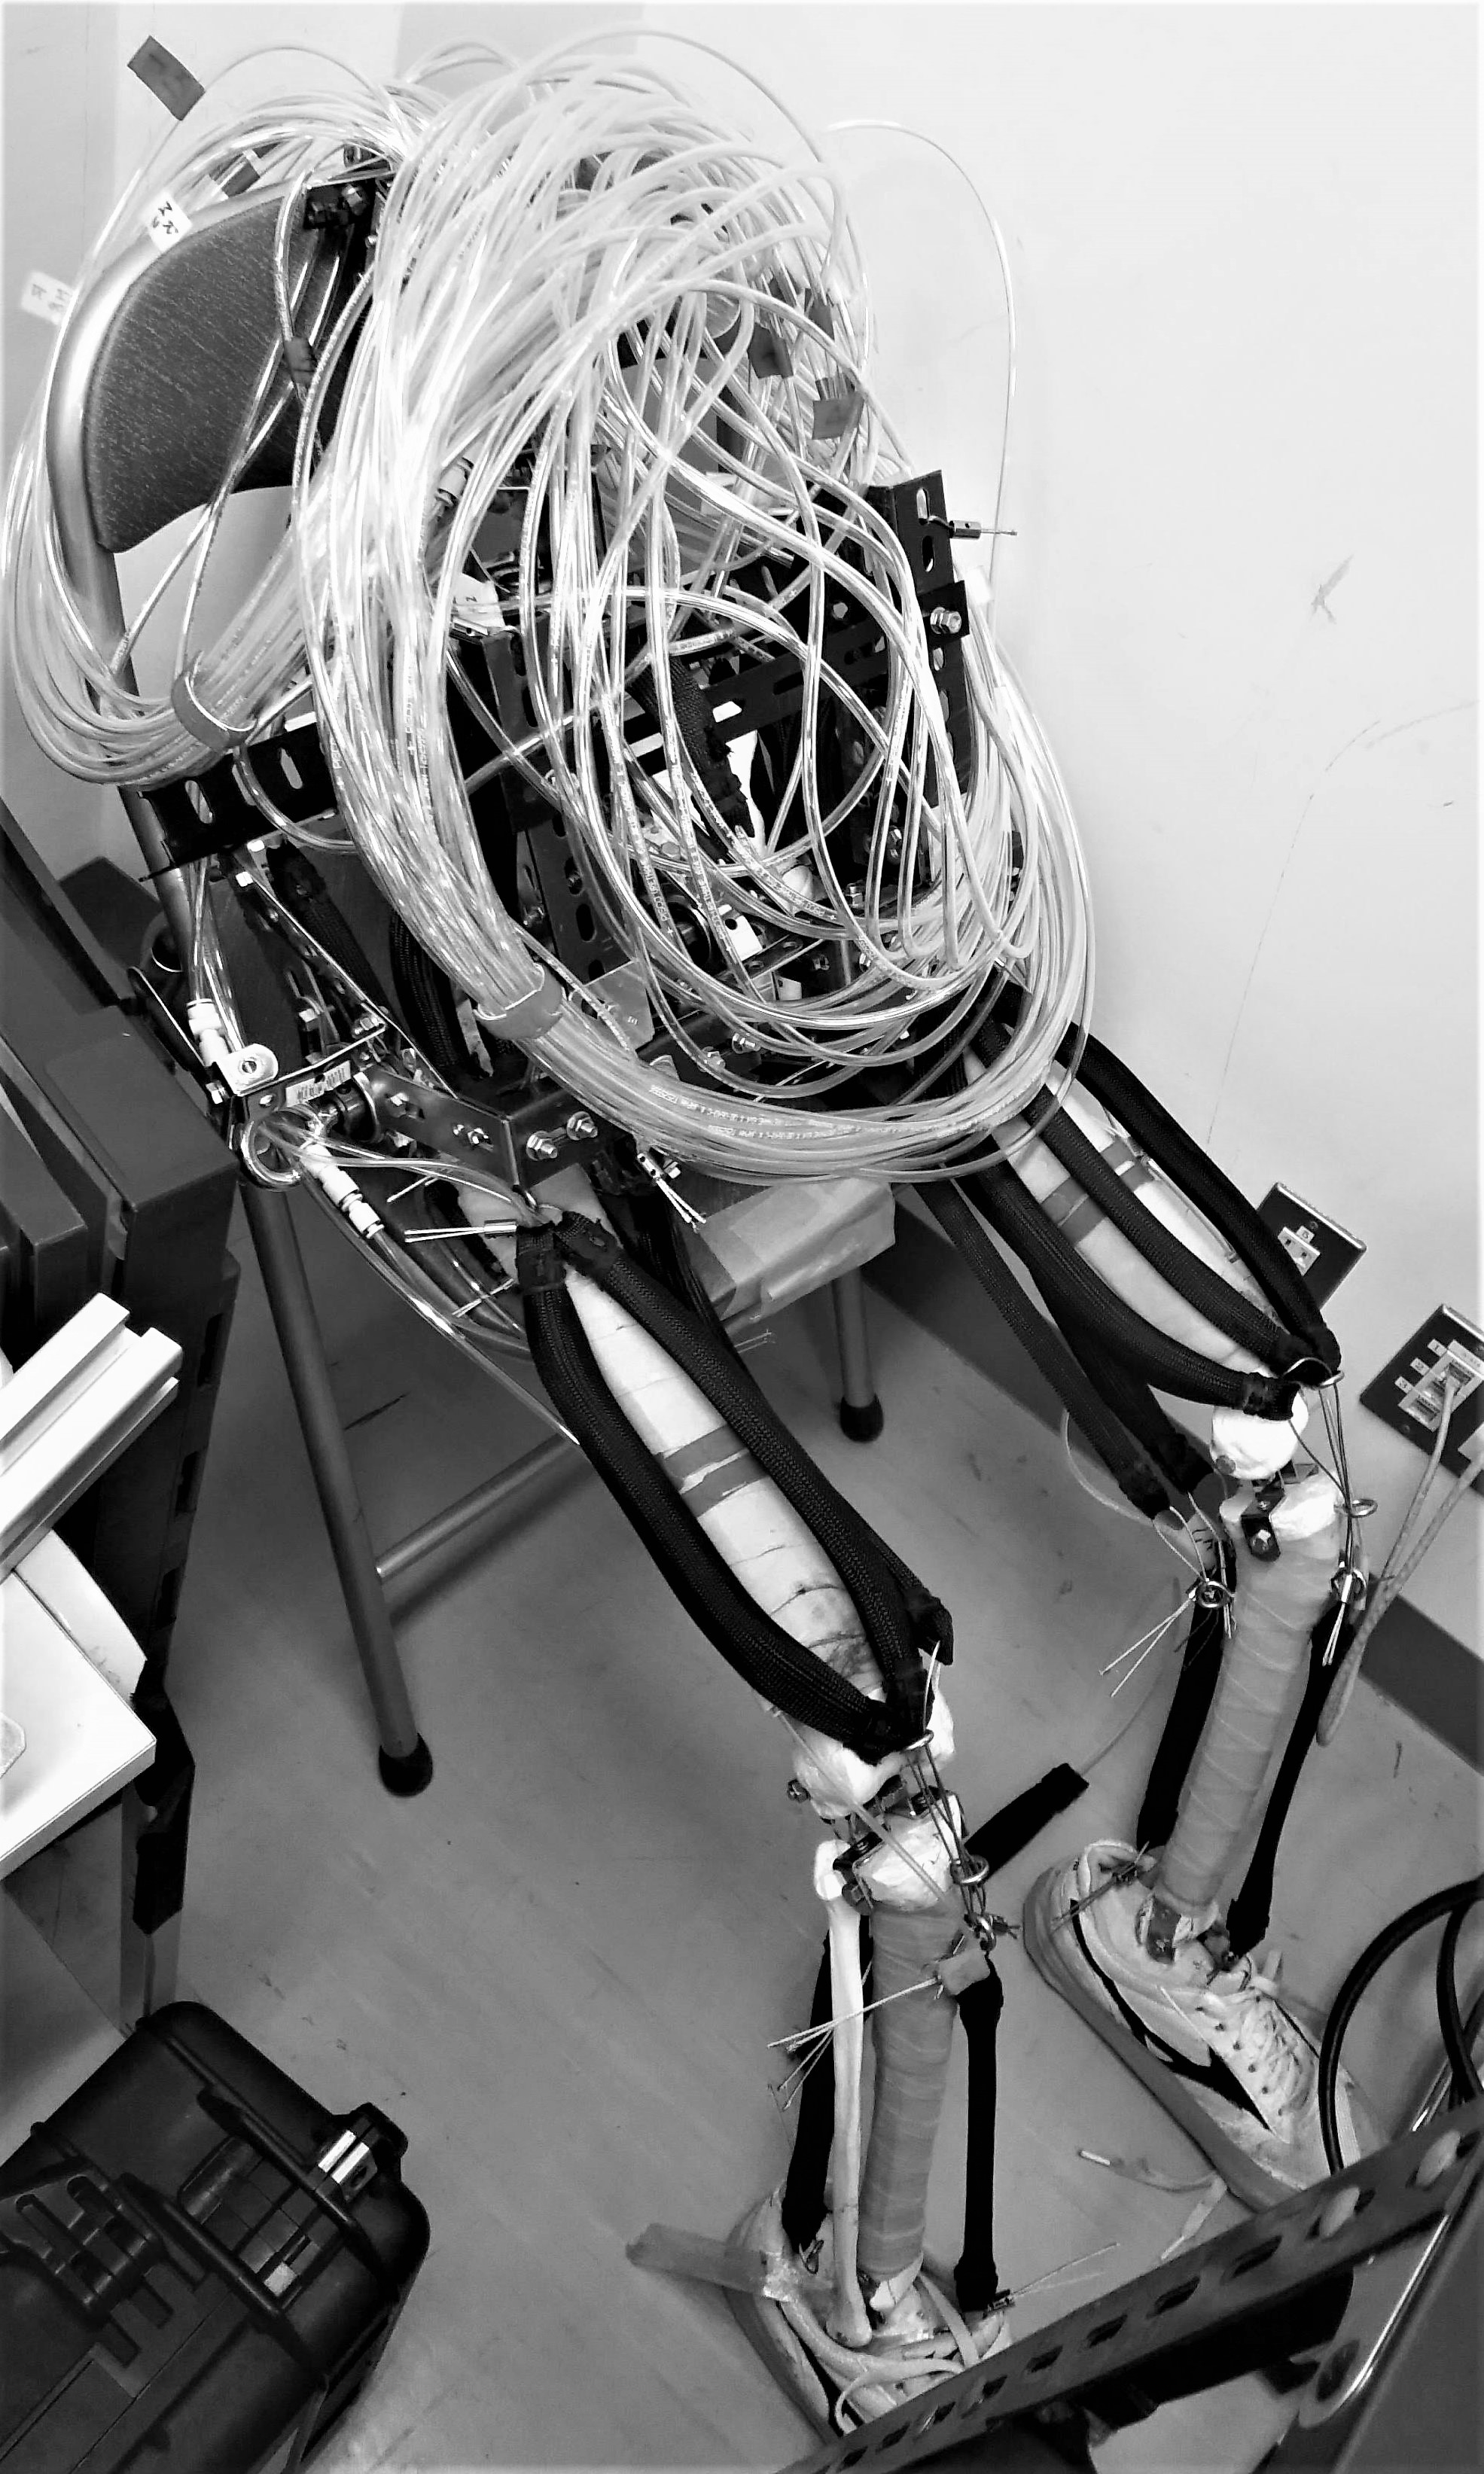
\includegraphics[width=5cm]{2nd.jpg}
        \caption{2機目2足歩行ロボット}
    \end{figure} %ここまではとりあえず校閲完了。

    現在は研究室におけるこれらの経験を基に空気圧人工筋を用いた2足ロボット3号機の製作を行っております。3機目の2足歩行ロボットを製作する目的として、関節自由度の向上・ひずみゲージを用いたセンサフィードバック・人をコントローラーとした姿勢制御としています。まず、自由度の向上に関しまして、従来は大腿骨と骨盤の間の自由度はピッチ方向のみの1自由度でした。また、足首周りに関しましても脛骨と足との自由度は足をピッチ方向のみの1自由度でした。これに対して、新造する構造においてそれぞれの関節にロール、ヨー方向の自由度を加えより人間に近づけたロボットになると考えられます。次に、ひずみゲージを用いたセンサフィードバックに関して、従来は筋シナジー情報を基にロボットを動作させておりフィードバックは行っていませんでした。これでは各筋肉のひずみ情報を得ることができず筋肉が無理な動作をした際の人間の反射的動作を再現することが出来ませんでした。また、ロボットにおける筋シナジー情報を得ることができませんでした。これらのことを改善するため、空気圧人工筋の各筋にひずみゲージを設置し各筋のひずみ情報を得ることとしました。このことより、ひずみ情報より導出される筋シナジー情報をフィードバックすることによりロボットの制御が正確に行われると考えられます。最後に人をコントローラーとした姿勢制御行うことに関して、従来は人間の筋シナジー情報を一方的に流し込むだけでその結果ロボットに出力された状態が人間にフィードバックされることはありませんでした。もし、人間にロボットの姿勢制御情報をフィードバックすることができれば自身で姿勢制御することが困難な方への姿勢補助の一端になると考えられます。従来でのこのタイプのロボットは外骨格型のセンサを用いて人間の動作を測定したものが存在します。ただ、外骨格型は人間に対して大きな器具を体に装着する必要があります。一方で今回研究で行おうとしている筋電情報より得られる筋シナジー情報を用いる方法では軽量な測定器具で人間の筋シナジー情報を得ることができ操縦者への負担が軽減すると考えられます。機体の製作に関し、骨格製作担当2名、空気圧関連製作担当1名、電装・制御担当1名に役割分担してチームで製作を行ってます。私はその中で電装・制御を担当してひずみ情報を用いたフィードバックシステムの製作、ロボットより人への姿勢情報フィードバックシステムの製作を行っています。

    続いて、もう一つの私が行っている研究である機能的電気刺激(FES)を用いた下肢の身体制御に関して以下に説明を示します。弊研究室では深部筋であるヒラメ筋に対して干渉波を用いた電気刺激によって動作介入を行うことが従来の研究で行えることが分かりました。この知見を活かし前脛骨筋に電気刺激を加え、足首のピッチ方向に電気刺激を用いて力を加えることが可能になりました。このことより足首のピッチ方向の剛性を高めることができます。また、同様な電気刺激を加えることで足首のロール、ヨー方向の制御も行えると考えられます。このことにより、自分自身で足首の動作が困難な麻痺患者さんに対しそのような姿勢制御介入を行うことで姿勢補助、さらには足首周りの機能回復が見込めると考えられ、本研究を進めています。

    \section{課題2今後取り組みたい研究内容に関して}
    私は貴学に合格いたしましたらてロボティクス研究室への所属を希望します。その主な理由といたしまして、人型ロボットの制御をよりロバスト性の高い、人らしい安定した動きにしたいと考えて現在研究を進めており、「視覚と行動計画を伴うヒューマノイドロボットのサービス提供」といった貴学のロボティクス研究室にて行われている研究が非常に合致していると思われるからです。

    2005年に愛知県にて開催されました「愛・地球博」にてロボットが実生活に浸透するのは遠い未来ではなく近い将来の話であるといった印象を受けました。しかし、それから14年程経過した現在、一部は実生活への導入が進みましたが、人型ロボットに関しては導入が特に遅れていると考えられます。加えて、現在、日本は少子化が進行した状態で超高齢社会となりました。その様な現状、社会における働き手不足が深刻化すると叫ばれています。その中、ロバスト性の高い人型ロボットが安価で存在することができれば人間の仕事の一部肩代わりするのではないかと強く思います。さらに、現在の研究内容や分野に近く現在自身の研究で学習している下肢の運動制御に関する知見を活かすことできると考えらるからです。

    以上の理由より、貴学へ入学いたしましたら高いロバスト性を持った人らしい動作が可能な人型ロボットの姿勢動作制御に関する研究を行いたいと考えます。
\end{document}